\documentclass[11pt,preprint]{elsarticle}

\usepackage{lmodern}
%%%% My spacing
\usepackage{setspace}
\setstretch{1.2}
\DeclareMathSizes{12}{14}{10}{10}

% Wrap around which gives all figures included the [H] command, or places it "here". This can be tedious to code in Rmarkdown.
\usepackage{float}
\let\origfigure\figure
\let\endorigfigure\endfigure
\renewenvironment{figure}[1][2] {
    \expandafter\origfigure\expandafter[H]
} {
    \endorigfigure
}

\let\origtable\table
\let\endorigtable\endtable
\renewenvironment{table}[1][2] {
    \expandafter\origtable\expandafter[H]
} {
    \endorigtable
}


\usepackage{ifxetex,ifluatex}
\usepackage{fixltx2e} % provides \textsubscript
\ifnum 0\ifxetex 1\fi\ifluatex 1\fi=0 % if pdftex
  \usepackage[T1]{fontenc}
  \usepackage[utf8]{inputenc}
\else % if luatex or xelatex
  \ifxetex
    \usepackage{mathspec}
    \usepackage{xltxtra,xunicode}
  \else
    \usepackage{fontspec}
  \fi
  \defaultfontfeatures{Mapping=tex-text,Scale=MatchLowercase}
  \newcommand{\euro}{€}
\fi

\usepackage{amssymb, amsmath, amsthm, amsfonts}

\def\bibsection{\section*{References}} %%% Make "References" appear before bibliography


\usepackage[numbers]{natbib}

\usepackage{longtable}
\usepackage[margin=2.3cm,bottom=2cm,top=2.5cm, includefoot]{geometry}
\usepackage{fancyhdr}
\usepackage[bottom, hang, flushmargin]{footmisc}
\usepackage{graphicx}
\numberwithin{equation}{section}
\numberwithin{figure}{section}
\numberwithin{table}{section}
\setlength{\parindent}{0cm}
\setlength{\parskip}{1.3ex plus 0.5ex minus 0.3ex}
\usepackage{textcomp}
\renewcommand{\headrulewidth}{0.2pt}
\renewcommand{\footrulewidth}{0.3pt}

\usepackage{array}
\newcolumntype{x}[1]{>{\centering\arraybackslash\hspace{0pt}}p{#1}}

%%%%  Remove the "preprint submitted to" part. Don't worry about this either, it just looks better without it:
\makeatletter
\def\ps@pprintTitle{%
  \let\@oddhead\@empty
  \let\@evenhead\@empty
  \let\@oddfoot\@empty
  \let\@evenfoot\@oddfoot
}
\makeatother

 \def\tightlist{} % This allows for subbullets!

\usepackage{hyperref}
\hypersetup{breaklinks=true,
            bookmarks=true,
            colorlinks=true,
            citecolor=blue,
            urlcolor=blue,
            linkcolor=blue,
            pdfborder={0 0 0}}


% The following packages allow huxtable to work:
\usepackage{siunitx}
\usepackage{multirow}
\usepackage{hhline}
\usepackage{calc}
\usepackage{tabularx}
\usepackage{booktabs}
\usepackage{caption}


\newenvironment{columns}[1][]{}{}

\newenvironment{column}[1]{\begin{minipage}{#1}\ignorespaces}{%
\end{minipage}
\ifhmode\unskip\fi
\aftergroup\useignorespacesandallpars}

\def\useignorespacesandallpars#1\ignorespaces\fi{%
#1\fi\ignorespacesandallpars}

\makeatletter
\def\ignorespacesandallpars{%
  \@ifnextchar\par
    {\expandafter\ignorespacesandallpars\@gobble}%
    {}%
}
\makeatother


% definitions for citeproc citations
\NewDocumentCommand\citeproctext{}{}
\NewDocumentCommand\citeproc{mm}{%
\begingroup\def\citeproctext{#2}\cite{#1}\endgroup}
\makeatletter
% allow citations to break across lines
\let\@cite@ofmt\@firstofone
% avoid brackets around text for \cite:
\def\@biblabel#1{}
\def\@cite#1#2{{#1\if@tempswa , #2\fi}}
\makeatother
\newlength{\cslhangindent}
\setlength{\cslhangindent}{1.5em}
\newlength{\csllabelwidth}
\setlength{\csllabelwidth}{3em}
\newenvironment{CSLReferences}[2] % #1 hanging-indent, #2 entry-spacing
{\begin{list}{}{%
	\setlength{\itemindent}{0pt}
	\setlength{\leftmargin}{0pt}
	\setlength{\parsep}{0pt}
	% turn on hanging indent if param 1 is 1
	\ifodd #1
	\setlength{\leftmargin}{\cslhangindent}
	\setlength{\itemindent}{-1\cslhangindent}
	\fi
	% set entry spacing
	\setlength{\itemsep}{#2\baselineskip}}}
{\end{list}}

\usepackage{calc}
\newcommand{\CSLBlock}[1]{\hfill\break\parbox[t]{\linewidth}{\strut\ignorespaces#1\strut}}
\newcommand{\CSLLeftMargin}[1]{\parbox[t]{\csllabelwidth}{\strut#1\strut}}
\newcommand{\CSLRightInline}[1]{\parbox[t]{\linewidth - \csllabelwidth}{\strut#1\strut}}
\newcommand{\CSLIndent}[1]{\hspace{\cslhangindent}#1}


\urlstyle{same}  % don't use monospace font for urls
\setlength{\parindent}{0pt}
\setlength{\parskip}{6pt plus 2pt minus 1pt}
\setlength{\emergencystretch}{3em}  % prevent overfull lines
\setcounter{secnumdepth}{5}

%%% Use protect on footnotes to avoid problems with footnotes in titles
\let\rmarkdownfootnote\footnote%
\def\footnote{\protect\rmarkdownfootnote}
\IfFileExists{upquote.sty}{\usepackage{upquote}}{}

%%% Include extra packages specified by user
\usepackage{lscape}\usepackage{booktabs}
\usepackage{longtable}
\usepackage{array}
\usepackage{multirow}
\usepackage{wrapfig}
\usepackage{float}
\usepackage{colortbl}
\usepackage{pdflscape}
\usepackage{tabu}
\usepackage{threeparttable}
\usepackage{threeparttablex}
\usepackage[normalem]{ulem}
\usepackage{makecell}
\usepackage{xcolor}

%%% Hard setting column skips for reports - this ensures greater consistency and control over the length settings in the document.
%% page layout
%% paragraphs
\setlength{\baselineskip}{12pt plus 0pt minus 0pt}
\setlength{\parskip}{12pt plus 0pt minus 0pt}
\setlength{\parindent}{0pt plus 0pt minus 0pt}
%% floats
\setlength{\floatsep}{12pt plus 0 pt minus 0pt}
\setlength{\textfloatsep}{20pt plus 0pt minus 0pt}
\setlength{\intextsep}{14pt plus 0pt minus 0pt}
\setlength{\dbltextfloatsep}{20pt plus 0pt minus 0pt}
\setlength{\dblfloatsep}{14pt plus 0pt minus 0pt}
%% maths
\setlength{\abovedisplayskip}{12pt plus 0pt minus 0pt}
\setlength{\belowdisplayskip}{12pt plus 0pt minus 0pt}
%% lists
\setlength{\topsep}{10pt plus 0pt minus 0pt}
\setlength{\partopsep}{3pt plus 0pt minus 0pt}
\setlength{\itemsep}{5pt plus 0pt minus 0pt}
\setlength{\labelsep}{8mm plus 0mm minus 0mm}
\setlength{\parsep}{\the\parskip}
\setlength{\listparindent}{\the\parindent}
%% verbatim
\setlength{\fboxsep}{5pt plus 0pt minus 0pt}



\begin{document}



\begin{frontmatter}  %

\title{Beyond Tit for Tat: A Deep Dive into Strategy and Social
Preferences}

% Set to FALSE if wanting to remove title (for submission)




\author[Add1]{Liam Andrew Beattie}
\ead{22562435@sun.ac.za}

\author[Add1]{Abdul Qaadir Cassiem}
\ead{20863667@sun.ac.za}




\address[Add1]{Microeconomics 871, Stellenbosch University, South
Africa}



\vspace{1cm}





\vspace{0.5cm}

\end{frontmatter}

\setcounter{footnote}{0}



%________________________
% Header and Footers
%%%%%%%%%%%%%%%%%%%%%%%%%%%%%%%%%
\pagestyle{fancy}
\chead{}
\rhead{}
\lfoot{}
\rfoot{\footnotesize Page \thepage}
\lhead{}
%\rfoot{\footnotesize Page \thepage } % "e.g. Page 2"
\cfoot{}

%\setlength\headheight{30pt}
%%%%%%%%%%%%%%%%%%%%%%%%%%%%%%%%%
%________________________

\headsep 35pt % So that header does not go over title




\section{\texorpdfstring{Introduction
\label{Introduction}}{Introduction }}\label{introduction}

The phrase horses for courses alludes to the fact that a racehorse
performs best on a racecourse to which it is specifically suited. More
generally this idiom is used to express that certain tools and
strategies are better suited over others depending on the task or
situations at hand. In the context of the repeated prisoners' dilemma,
the strategy of Tit for Tat (TfT), where one mimics their opponent's
previous move, reigns supreme and is best suited over others for the
situation at hand.

This paper investigates strategic behaviour in the repeated Prisoner's
Dilemma by conducting a tournament inspired by Axelrod (1980) but
expands the original framework by including distinct strategies. These
strategies, categorized into cooperative, defecting, random, and
adaptive types, play against each other in 200 rounds of the Prisoner's
Dilemma, allowing for a comprehensive evaluation of their performance.
By considering both standard scenarios and environments with varying
levels of social preferences, this study explores how different
strategies fare in diverse settings, particularly focusing on the
adaptability and effectiveness of Tit for Tat (TfT) variants, which have
historically been prominent in such tournaments.

\section{\texorpdfstring{Literature
Review\label{litreview}}{Literature Review}}\label{literature-review}

The exploration of strategy choices within the framework of the
prisoner's dilemma has garnered extensive attention in recent
literature. Axelrod (1980) foundational work emphasized effective
strategies in iterated scenarios, sparking a wealth of research on
strategic behaviour in repeated interactions. His tournament studies
laid the groundwork for understanding how cooperation can emerge in
repeated prisoner's dilemmas through strategies like Tit for Tat (TfT)
and other forms of reciprocity. This exploration of cooperative
behaviour in an inherently competitive framework has been expanded by
various scholars, each contributing unique insights into how individuals
and institutions behave when faced with the tension between cooperation
and defection.

Recent studies, such as that by Bó \& Fréchette (2019), have focused on
the strategic complexity observed in infinitely repeated games. They
provide empirical evidence that players in these settings are highly
adaptive, often switching strategies depending on the payoffs and the
perceived actions of their opponents. In contrast, Breitmoser (2015)
questions the reciprocity-based models that dominate much of the
literature, suggesting that while cooperation is often observed, it may
not always stem from reciprocal motivations. Breitmoser (2015) finds
that in many cases, cooperation might emerge from individual incentives
structured by the game's dynamics, rather than a direct desire to
reciprocate.

A significant portion of the literature has also addressed the
challenges of finite versus infinite iterations of the dilemma. Kreps,
Milgrom, Roberts \& Wilson (1982) introduced the idea that even in
finitely repeated games, players may behave as though they are in an
infinite game, cooperating for fear of future retaliation, despite the
known endpoint. This idea challenges the strict predictions of defection
in the final stages of finitely repeated games and has been explored
further by Embrey, Fréchette \& Yuksel (2018), who conducted laboratory
experiments to observe how players adapt their strategies in finite
games. Their findings support the hypothesis that cooperation can
persist under certain conditions, even in games with a clear end.

Adding to the complexity of the strategic decision-making landscape,
Romero \& Rosokha (2018) investigated the cognitive processes behind
strategy construction in indefinite games, emphasizing how players use
heuristics and simplified mental models to navigate the uncertainty of
the game's length. This aligns with Farrell \& Ware (1989) earlier work
on evolutionary stability, where they explored how long-term strategies
evolve to withstand deviations from equilibrium behaviours.

From a computational perspective, García \& Veelen (2018) utilized
simulations to demonstrate that no single strategy could consistently
dominate in the repeated prisoner's dilemma, suggesting that
adaptability and context-dependent strategy selection are key to success
in such settings. Similarly, Gaudesi, Piccolo, Squillero \& Tonda (2016)
leveraged evolutionary modelling techniques to demonstrate how
strategies evolve, competing in a dynamic landscape shaped by both
cooperation and competition.

The link between theoretical models and real-world applications has also
been a point of focus. Lange \& Baylor (2007) developed computerized
tournaments to teach the mechanics of the repeated prisoner's dilemma,
blending theory with practice and providing insights into how strategic
choices might play out in educational settings. Such studies highlight
the importance of teaching and learning mechanisms in understanding
strategic behaviour in social dilemmas. Taken together, the contemporary
literature on strategy selection in the prisoner's dilemma underscores
the complexity of human decision-making in repeated interactions.

\section{The Standard Prisoners
Dilemma}\label{the-standard-prisoners-dilemma}

This paper conducts a tournament modelled after Axelrod (1980) but
incorporates a wider array of strategies. A total of 25 strategies are
used in this repeated Prisoner's Dilemma tournament. These strategies
are categorized in Table 3.1 according to their types. Some strategies
always cooperate or always defect, while others, called random
strategies, cooperate with a set probability. For example, Random 90\%
cooperates 90\% of the time and defects 10\% of the time. Strategies
extracted from the literature are marked with references in brackets
next to their names. Those without references are new strategies
introduced in this paper, each of which will be explained in detail.

\renewcommand{\arraystretch}{1.2} % Adjust row spacing
\begin{table}[ht]
\centering
\tiny % Reduces font size for compactness
\begin{tabular}{|>{\centering\arraybackslash}p{2cm}|>{\centering\arraybackslash}p{2cm}|>{\centering\arraybackslash}p{2cm}|>{\centering\arraybackslash}p{2cm}|>{\centering\arraybackslash}p{2cm}|>{\centering\arraybackslash}p{2cm}|>{\centering\arraybackslash}p{2cm}|}
\hline
\textbf{Always Strategies} & \textbf{Tit for Tat Variants} & \textbf{Win-Stay/ Lose-Switch} & \textbf{Punishment-Based} & \textbf{Adaptive/ Adjusting} & \textbf{Gradient/ Probability-Based} & \textbf{Random Strategies} \\
\hline
Always Cooperate & Tit for Tat & Pavlov & Grim Trigger & Adaptive Defector & Progressive Cooperator & Random 10\% \\
Always Defect & Tit for Two Tats & & Bully & Adaptive Peacekeeper & Diminishing Cooperator & Random 25\% \\
& Tit for Tat with Randomisation & & Retaliatory Defector & Probing Adjuster & Bounded Gradient & Random 50\% \\
& Tit for Tat with Forgiveness & & & Forgiving Tester & Recent Gradient & Random 75\% \\
& & & & Prober & & Random 90\% \\
& & & & Cautious Rebuilder & & \\
\hline
\end{tabular}
\caption{Categorisation of Strategy Types Used in the Prisoner's Dilemma Tournament}
\end{table}

One such strategy is Retaliatory Defector. It begins by cooperating but
defects for two rounds if its opponent defects. After two rounds, if the
opponent resumes cooperation, Retaliatory Defector will also return to
cooperating. Another strategy, Adaptive Defector, also starts by
cooperating, but thereafter assesses the opponent's behaviour over the
last five rounds. If the opponent has defected more than 40\% of the
time, Adaptive Defector will defect; otherwise, it continues to
cooperate. Adaptive Peacekeeper focuses on maintaining cooperation while
testing the opponent's behaviour periodically. It starts by cooperating
but defects every sixth round to probe the opponent's reaction. If the
opponent defects more than twice consecutively after these probes,
Adaptive Peacekeeper responds with defection. However, if both players
defected in the previous round, the strategy returns to cooperation,
signalling a willingness to restore collaboration.

Probing Adjuster is another adaptive strategy. It begins by cooperating
but alters its behaviour based on the opponent's past actions. If the
opponent defects three times in a row, Probing Adjuster responds by
defecting as well. However, if both players defected in the previous
round, it tries to re-establish cooperation by cooperating again. If the
opponent cooperates after the player defects, the player will continue
defecting, exploiting the opponent's leniency. Additionally, if the
player cooperates while the opponent cooperates, the player switches to
defection to test the opponent's reaction to a shift in strategy.

Prober tests the opponent's resilience to defection by defecting for
three consecutive rounds if the opponent defects. It always begins with
cooperation, but when an opponent defects, Prober immediately retaliates
with three rounds of defection before returning to cooperation. This
approach aims to probe the opponent's willingness to adjust their
behaviour in response to repeated defection while maintaining a
cooperative default when unprovoked.

Forgiving Tester emphasizes cooperation but incorporates occasional
defections to gauge the opponent's response. It begins by cooperating,
but every fourth round it defects. If the opponent defects three times
in a row, Forgiving Tester will retaliate by continuing to defect until
the opponent cooperates again. However, if the opponent cooperates after
a test defection, or if both players defect in the same round, Forgiving
Tester quickly forgives and returns to cooperation. This strategy
encourages long-term collaboration while punishing consistent
defections.

Cautious Rebuilder starts by cooperating and follows three rules in its
decision-making. First, if the opponent defects three times in a row,
Cautious Rebuilder will defect until the opponent cooperates again.
Second, if the opponent's last move was a defection but the opponent has
not defected three times consecutively, Cautious Rebuilder will
cooperate, trying to repair relations. Third, after every five rounds,
it will defect once to test the opponent's tolerance for defection. In
line with Axelrod (1980), each strategy plays against itself and every
other strategy once in the tournament. Each game consists of 200 rounds
of the repeated Prisoner's Dilemma, and the payoffs and outcomes are
recorded for every round. The strategy that accumulates the most points
after 200 rounds wins the individual game. The overall winner of the
tournament is the strategy that achieves the highest total points across
all games. The standard Prisoners Dilemma from Axelrod (1980) will be
played and is given in the table below:

\begin{table}[ht]
\centering
\begin{tabular}{|c|c|c|}
\hline
\textbf{Player 1 / Player 2} & \textbf{C (Cooperate)} & \textbf{D (Defect)} \\
\hline
\textbf{C (Cooperate)} & $(3, 3)$ & $(0, 5)$ \\
\hline
\textbf{D (Defect)} & $(5, 0)$ & $(1, 1)$ \\
\hline
\end{tabular}
\caption{Prisoner's Dilemma Payoff Matrix}
\end{table}

\subsection{Introducing Social
Preferences}\label{introducing-social-preferences}

This game is played the same as above except now Social Preferences are
taken into account. From-game adjustments are a bit different and it
considers the utility a player gets from the payoffs of its opponent.
The standard Prisoners Dilemma payoff Matrix with from-game adjustments
is given below:

\begin{table}[ht]
\centering
\begin{tabular}{|c|c|c|}
\hline
\textbf{Player 1 / Player 2} & \textbf{C (Cooperate)} & \textbf{D (Defect)} \\
\hline
\textbf{C (Cooperate)} & $(3(1-p) + 3p,     3(1-p) + 3p)$ & $(0(1-p) + 5p,     5(1-p)+0p)$ \\
\hline
\textbf{D (Defect)} & $(5(1-p) + 0p,    0(1-p) + 5p)$ & $((1-p) + p,     (1-p) + p)$ \\
\hline
\end{tabular}
\caption{Prisoner's Dilemma Payoff Matrix}
\end{table}

The level \emph{p} here is adapted from Charness \& Rabin (2002) who
created a utility function that captures various social preferences. In
essence, \emph{p} is how much you care about your opponent's pay-offs as
well as your own. This paper will conduct the tournament as above for a
range of \emph{p} values starting from \emph{p} = -1 where individuals
are status seeking to \emph{p} = 0.5 where individuals care half as much
about themselves as they do about others

\section{Game Results}\label{game-results}

\subsection{The Standard Prisoners Dilemma
Tournament}\label{the-standard-prisoners-dilemma-tournament}

After the conclusion of the tournament, most interestingly unlike
Axelrod (1980), this paper does not find Tft as the winner in the
standard Repeated Prisoners Dilemma. Table 4.1 gives the standard
tournament without social preferences. The winner of the tournament was
Probing Adjuster with 13575 points followed by Tft with Randomization
which had 12887 points and Bully coming in third with 12869 points. In
this game, Tft came fourth which leads us to believe similarly to
Axelrod (1980) that Tft may have won due to the other strategies in the
tournament. The winner of the Prisoners Dilemma is highly dependent on
the strategies in the tournament. Always Cooperate and Random 90\% came
in second last and last respectively. This is as expected as the
tournament included strategies that took advantage of other strategies
which always cooperated. Most interestingly, if the adaptive strategies
were removed then the Grim/Trigger strategy would have won the game.
Also, even though Probing Adjuster won the tournament, the group of
adaptive strategies as a whole performed worse than the group of Tit for
Tat variant strategies. This result shows the robustness of Tit for Tat
variants to perform well against both cooperators and defectors,
maintaining high scores overall.

\newpage

\begin{landscape}


\vfill
\begingroup\fontsize{5}{7}\selectfont

\begin{longtable}[t]{>{}l>{\raggedleft\arraybackslash}p{0.25cm}>{\raggedleft\arraybackslash}p{0.25cm}>{\raggedleft\arraybackslash}p{0.25cm}>{\raggedleft\arraybackslash}p{0.25cm}>{\raggedleft\arraybackslash}p{0.25cm}>{\raggedleft\arraybackslash}p{0.25cm}>{\raggedleft\arraybackslash}p{0.25cm}>{\raggedleft\arraybackslash}p{0.25cm}>{\raggedleft\arraybackslash}p{0.25cm}>{\raggedleft\arraybackslash}p{0.25cm}>{\raggedleft\arraybackslash}p{0.25cm}>{\raggedleft\arraybackslash}p{0.25cm}>{\raggedleft\arraybackslash}p{0.25cm}>{\raggedleft\arraybackslash}p{0.25cm}>{\raggedleft\arraybackslash}p{0.25cm}>{\raggedleft\arraybackslash}p{0.25cm}>{\raggedleft\arraybackslash}p{0.25cm}>{\raggedleft\arraybackslash}p{0.25cm}>{\raggedleft\arraybackslash}p{0.25cm}>{\raggedleft\arraybackslash}p{0.25cm}>{\raggedleft\arraybackslash}p{0.25cm}>{\raggedleft\arraybackslash}p{0.25cm}>{\raggedleft\arraybackslash}p{0.25cm}>{\raggedleft\arraybackslash}p{0.25cm}>{\raggedleft\arraybackslash}p{0.25cm}>{\raggedleft\arraybackslash}p{0.2cm}>{\raggedleft\arraybackslash}p{0.2cm}}
\caption{\label{tab:unnamed-chunk-3}Tournament Payoff Matrix for p= 0}\\
\toprule
\multicolumn{1}{c}{ } & \multicolumn{25}{c}{Payoff Against Other Strategies} & \multicolumn{1}{c}{Total} & \multicolumn{1}{c}{Rank} \\
\cmidrule(l{3pt}r{3pt}){2-26} \cmidrule(l{3pt}r{3pt}){27-27} \cmidrule(l{3pt}r{3pt}){28-28}
 & AC & AD & TfT & Tf2T & TfTF & TfTR & P & G/T & B & RD & ADe & APe & PA & FT & P & CR & PC & DC & BG & RG & R0.1 & R0.25 & R0.5 & R0.75 & R0.9 &  & \\
\midrule
\textbf{Always Cooperate} & 600 & 0 & 600 & 600 & 600 & 600 & 600 & 600 & 147 & 600 & 600 & 501 & 3 & 453 & 600 & 483 & 291 & 261 & 600 & 600 & 69 & 156 & 300 & 420 & 519 & \textcolor{blue}{\textbf{10803}} & \textcolor{red}{\textbf{24}}\\
\textbf{Always Defect} & 1000 & 200 & 204 & 208 & 276 & 204 & 204 & 204 & 396 & 992 & 204 & 212 & 208 & 212 & 1000 & 212 & 664 & 600 & 204 & 1000 & 276 & 392 & 648 & 792 & 896 & \textcolor{blue}{\textbf{11408}} & \textcolor{red}{\textbf{20}}\\
\textbf{Tit for Tat} & 600 & 199 & 600 & 600 & 600 & 600 & 600 & 600 & 346 & 600 & 600 & 567 & 399 & 551 & 600 & 561 & 441 & 426 & 600 & 600 & 250 & 344 & 432 & 531 & 580 & \textcolor{blue}{\textbf{12827}} & \textcolor{red}{\textbf{4}}\\
\textbf{Tit for Two Tats} & 600 & 198 & 600 & 600 & 600 & 600 & 600 & 600 & 296 & 600 & 600 & 501 & 298 & 453 & 600 & 483 & 372 & 370 & 600 & 600 & 244 & 288 & 394 & 480 & 548 & \textcolor{blue}{\textbf{12125}} & \textcolor{red}{\textbf{15}}\\
\textbf{Tit for Tat with Forgiveness} & 600 & 183 & 600 & 600 & 600 & 600 & 600 & 600 & 322 & 600 & 600 & 561 & 370 & 539 & 600 & 553 & 408 & 411 & 600 & 600 & 249 & 321 & 403 & 527 & 571 & \textcolor{blue}{\textbf{12618}} & \textcolor{red}{\textbf{8}}\\
\addlinespace
\textbf{Tit for Tat with Randomisation} & 600 & 199 & 600 & 600 & 600 & 600 & 600 & 600 & 346 & 600 & 600 & 567 & 399 & 551 & 600 & 561 & 422 & 436 & 600 & 600 & 252 & 357 & 478 & 542 & 577 & \textcolor{blue}{\textbf{12887}} & \textcolor{red}{\textbf{2}}\\
\textbf{Pavlov} & 600 & 199 & 600 & 600 & 600 & 600 & 600 & 600 & 346 & 600 & 600 & 567 & 399 & 551 & 600 & 561 & 453 & 434 & 600 & 600 & 243 & 325 & 442 & 519 & 582 & \textcolor{blue}{\textbf{12821}} & \textcolor{red}{\textbf{5}}\\
\textbf{Grim/Trigger} & 600 & 199 & 600 & 600 & 600 & 600 & 600 & 600 & 395 & 600 & 600 & 223 & 205 & 219 & 600 & 221 & 607 & 575 & 600 & 600 & 263 & 399 & 551 & 823 & 933 & \textcolor{blue}{\textbf{12813}} & \textcolor{red}{\textbf{6}}\\
\textbf{Bully} & 902 & 151 & 351 & 551 & 399 & 351 & 351 & 155 & 298 & 894 & 155 & 683 & 355 & 751 & 902 & 631 & 533 & 554 & 348 & 902 & 230 & 319 & 556 & 700 & 847 & \textcolor{blue}{\textbf{12869}} & \textcolor{red}{\textbf{3}}\\
\textbf{Retaliatory Defector} & 600 & 2 & 600 & 600 & 600 & 600 & 600 & 600 & 149 & 600 & 600 & 505 & 9 & 457 & 600 & 487 & 263 & 283 & 600 & 600 & 74 & 122 & 319 & 463 & 541 & \textcolor{blue}{\textbf{10874}} & \textcolor{red}{\textbf{23}}\\
\addlinespace
\textbf{Adaptive Defector} & 600 & 199 & 600 & 600 & 600 & 600 & 600 & 600 & 395 & 600 & 600 & 501 & 205 & 453 & 600 & 483 & 448 & 420 & 600 & 600 & 276 & 387 & 457 & 487 & 548 & \textcolor{blue}{\textbf{12459}} & \textcolor{red}{\textbf{10}}\\
\textbf{Adaptive Peacekeep} & 666 & 197 & 567 & 666 & 576 & 567 & 567 & 213 & 263 & 660 & 666 & 534 & 256 & 503 & 666 & 543 & 418 & 400 & 572 & 666 & 223 & 285 & 393 & 483 & 600 & \textcolor{blue}{\textbf{12150}} & \textcolor{red}{\textbf{14}}\\
\textbf{Probing Adjuster} & 998 & 198 & 404 & 553 & 436 & 404 & 404 & 205 & 345 & 989 & 205 & 591 & 400 & 557 & 998 & 643 & 587 & 544 & 325 & 998 & 264 & 369 & 549 & 719 & 890 & \textcolor{blue}{\textbf{13575}} & \textcolor{red}{\textbf{1}}\\
\textbf{Forgiving Tester} & 698 & 197 & 551 & 698 & 563 & 551 & 551 & 209 & 246 & 692 & 698 & 583 & 297 & 502 & 698 & 572 & 452 & 431 & 565 & 698 & 239 & 275 & 393 & 543 & 631 & \textcolor{blue}{\textbf{12533}} & \textcolor{red}{\textbf{9}}\\
\textbf{Prober} & 600 & 0 & 600 & 600 & 600 & 600 & 600 & 600 & 147 & 600 & 600 & 501 & 3 & 453 & 600 & 483 & 324 & 303 & 600 & 600 & 63 & 156 & 318 & 492 & 540 & \textcolor{blue}{\textbf{10983}} & \textcolor{red}{\textbf{21}}\\
\addlinespace
\textbf{Cautious Rebuilder} & 678 & 197 & 561 & 678 & 576 & 561 & 561 & 211 & 276 & 672 & 678 & 573 & 238 & 522 & 678 & 522 & 413 & 385 & 554 & 678 & 229 & 270 & 402 & 541 & 641 & \textcolor{blue}{\textbf{12295}} & \textcolor{red}{\textbf{11}}\\
\textbf{Progressive Cooperator} & 798 & 102 & 439 & 557 & 484 & 417 & 414 & 105 & 271 & 794 & 444 & 546 & 203 & 503 & 790 & 504 & 417 & 467 & 289 & 798 & 159 & 247 & 506 & 658 & 742 & \textcolor{blue}{\textbf{11654}} & \textcolor{red}{\textbf{18}}\\
\textbf{Deminishing Cooperator} & 784 & 109 & 438 & 536 & 454 & 432 & 447 & 141 & 263 & 799 & 410 & 543 & 235 & 487 & 818 & 522 & 499 & 431 & 619 & 798 & 176 & 262 & 435 & 653 & 715 & \textcolor{blue}{\textbf{12006}} & \textcolor{red}{\textbf{16}}\\
\textbf{Bounded Gradient} & 600 & 199 & 600 & 600 & 600 & 600 & 600 & 600 & 342 & 600 & 600 & 564 & 245 & 520 & 600 & 545 & 513 & 325 & 600 & 600 & 273 & 374 & 442 & 540 & 566 & \textcolor{blue}{\textbf{12648}} & \textcolor{red}{\textbf{7}}\\
\textbf{Recent Gradient} & 600 & 0 & 600 & 600 & 600 & 600 & 600 & 600 & 147 & 600 & 600 & 501 & 3 & 453 & 600 & 483 & 285 & 312 & 600 & 600 & 84 & 150 & 291 & 462 & 549 & \textcolor{blue}{\textbf{10920}} & \textcolor{red}{\textbf{22}}\\
\addlinespace
\textbf{Random 10\%} & 960 & 184 & 255 & 340 & 354 & 251 & 267 & 182 & 381 & 966 & 184 & 325 & 266 & 375 & 938 & 351 & 589 & 560 & 242 & 976 & 238 & 381 & 542 & 812 & 882 & \textcolor{blue}{\textbf{11801}} & \textcolor{red}{\textbf{17}}\\
\textbf{Random 25\%} & 886 & 149 & 367 & 452 & 415 & 353 & 354 & 156 & 329 & 900 & 233 & 533 & 314 & 406 & 900 & 508 & 553 & 498 & 353 & 904 & 216 & 364 & 564 & 695 & 809 & \textcolor{blue}{\textbf{12211}} & \textcolor{red}{\textbf{13}}\\
\textbf{Random 50\%} & 794 & 100 & 428 & 654 & 497 & 460 & 469 & 105 & 260 & 803 & 480 & 634 & 259 & 576 & 806 & 565 & 427 & 467 & 448 & 806 & 188 & 257 & 445 & 625 & 710 & \textcolor{blue}{\textbf{12263}} & \textcolor{red}{\textbf{12}}\\
\textbf{Random 75\%} & 714 & 59 & 538 & 656 & 538 & 525 & 536 & 77 & 217 & 692 & 643 & 609 & 151 & 536 & 726 & 574 & 377 & 358 & 530 & 704 & 107 & 224 & 325 & 532 & 660 & \textcolor{blue}{\textbf{11608}} & \textcolor{red}{\textbf{19}}\\
\textbf{Random 90\%} & 630 & 21 & 570 & 634 & 581 & 572 & 577 & 64 & 169 & 628 & 631 & 541 & 94 & 471 & 620 & 517 & 319 & 324 & 555 & 634 & 76 & 147 & 329 & 460 & 591 & \textcolor{blue}{\textbf{10755}} & \textcolor{red}{\textbf{25}}\\
\bottomrule
\end{longtable}
\endgroup{}

\vfill

\end{landscape}

\subsection{The Prisoners Dilemma Tournament with Social
Preferences}\label{the-prisoners-dilemma-tournament-with-social-preferences}

Table 4.2 gives the standings of the tournament across different social
preferences. The rankings of strategies change across these different
values of \emph{p}, illustrating how varying degrees of altruism or
hostility affect the success of each strategy. Notably Always Cooperate
improves its ranking as \emph{p} increases, moving from 25th at \emph{p}
= -0.1 to 1st when \emph{p} = 0.45, showing that cooperative strategies
perform better in environments where mutual benefit is prioritized.
Always Defect, conversely, declines in rank as \emph{p} increases,
indicating that purely selfish strategies are less effective when
players care about the well-being of others. Tit for Tat maintains a
relatively stable performance across various \emph{p} values, reflecting
its robustness as a strategy that adapts well to different social
preferences. This holds for the TfT variations in general. Probing
Adjuster, which ranked first when \emph{p} = -0.1, drops significantly
as p increases, indicating that more complex strategies designed for
selfish environments are less effective in altruistic settings.

\begin{table}[!h]
\centering
\caption{\label{tab:unnamed-chunk-4}Strategy Rankings Across Different p Values}
\centering
\resizebox{\ifdim\width>\linewidth\linewidth\else\width\fi}{!}{
\fontsize{5}{7}\selectfont
\begin{tabular}[t]{>{\centering\arraybackslash}p{4cm}>{\centering\arraybackslash}p{0.7cm}>{\centering\arraybackslash}p{0.7cm}>{\centering\arraybackslash}p{0.7cm}>{\centering\arraybackslash}p{0.7cm}>{\centering\arraybackslash}p{0.7cm}>{\centering\arraybackslash}p{0.7cm}>{\centering\arraybackslash}p{0.7cm}>{\centering\arraybackslash}p{0.7cm}>{\centering\arraybackslash}p{0.7cm}>{\centering\arraybackslash}p{0.7cm}>{\centering\arraybackslash}p{0.7cm}>{\centering\arraybackslash}p{0.7cm}>{\centering\arraybackslash}p{0.7cm}}
\toprule
\multicolumn{1}{c}{ } & \multicolumn{13}{c}{p Values} \\
\cmidrule(l{3pt}r{3pt}){2-14}
Strategy & -0.1 & -0.05 & 0 & 0.05 & 0.1 & 0.15 & 0.2 & 0.25 & 0.3 & 0.35 & 0.4 & 0.45 & 0.5\\
\midrule
\textbf{Always Cooperate} & 25 & 24 & 25 & 22 & 19 & 19 & 14 & 10 & 4 & 4 & 4 & 1 & 3\\
\textbf{Always Defect} & 15 & 18 & 20 & 25 & 25 & 25 & 25 & 25 & 25 & 25 & 25 & 25 & 25\\
\textbf{Tit for Tat} & 5 & 4 & 3 & 3 & 3 & 1 & 2 & 4 & 5 & 8 & 8 & 11 & 9\\
\textbf{Tit for Two Tats} & 18 & 16 & 15 & 13 & 11 & 7 & 6 & 5 & 9 & 6 & 6 & 6 & 6\\
\textbf{Tit for Tat with Forgiveness} & 10 & 8 & 7 & 5 & 4 & 4 & 4 & 3 & 6 & 7 & 7 & 7 & 8\\
\midrule
\textbf{Tit for Tat with Randomisation} & 4 & 6 & 5 & 4 & 1 & 2 & 1 & 2 & 7 & 9 & 10 & 8 & 11\\
\textbf{Pavlov} & 6 & 5 & 2 & 2 & 2 & 3 & 3 & 1 & 8 & 10 & 9 & 9 & 10\\
\textbf{Grim/Trigger} & 3 & 3 & 4 & 7 & 9 & 9 & 15 & 18 & 18 & 18 & 19 & 19 & 20\\
\textbf{Bully} & 2 & 2 & 8 & 8 & 10 & 15 & 20 & 21 & 22 & 21 & 21 & 21 & 21\\
\textbf{Retaliatory Defector} & 23 & 21 & 22 & 20 & 17 & 16 & 10 & 9 & 1 & 3 & 2 & 3 & 4\\
\midrule
\textbf{Adaptive Defector} & 12 & 10 & 11 & 9 & 7 & 8 & 7 & 11 & 13 & 13 & 13 & 13 & 14\\
\textbf{Adaptive Peacekeep} & 17 & 14 & 13 & 14 & 13 & 10 & 12 & 13 & 15 & 14 & 14 & 14 & 13\\
\textbf{Probing Adjuster} & 1 & 1 & 1 & 1 & 5 & 12 & 19 & 20 & 21 & 22 & 22 & 22 & 22\\
\textbf{Forgiving Tester} & 9 & 9 & 9 & 10 & 8 & 6 & 8 & 12 & 14 & 15 & 15 & 16 & 16\\
\textbf{Prober} & 21 & 22 & 24 & 24 & 21 & 17 & 13 & 8 & 3 & 1 & 1 & 2 & 1\\
\midrule
\textbf{Cautious Rebuilder} & 14 & 12 & 12 & 12 & 12 & 11 & 9 & 16 & 16 & 16 & 16 & 15 & 15\\
\textbf{Progressive Cooperator} & 19 & 20 & 17 & 18 & 23 & 22 & 22 & 22 & 20 & 20 & 20 & 20 & 19\\
\textbf{Deminishing Cooperator} & 16 & 17 & 16 & 15 & 16 & 20 & 21 & 19 & 19 & 19 & 18 & 18 & 18\\
\textbf{Bounded Gradient} & 8 & 7 & 6 & 6 & 6 & 5 & 5 & 6 & 10 & 11 & 12 & 12 & 12\\
\textbf{Recent Gradient} & 22 & 25 & 23 & 21 & 18 & 18 & 11 & 7 & 2 & 2 & 3 & 4 & 2\\
\midrule
\textbf{Random 10\%} & 11 & 15 & 18 & 19 & 24 & 24 & 24 & 24 & 24 & 24 & 24 & 24 & 24\\
\textbf{Random 25\%} & 7 & 13 & 14 & 16 & 19 & 23 & 23 & 23 & 23 & 23 & 23 & 23 & 23\\
\textbf{Random 50\%} & 13 & 11 & 10 & 11 & 14 & 13 & 18 & 17 & 17 & 17 & 17 & 17 & 17\\
\textbf{Random 75\%} & 20 & 19 & 19 & 17 & 15 & 14 & 16 & 15 & 12 & 12 & 11 & 10 & 7\\
\textbf{Random 90\%} & 24 & 23 & 21 & 23 & 22 & 21 & 17 & 14 & 11 & 5 & 5 & 5 & 5\\
\bottomrule
\end{tabular}}
\end{table}

Figure \ref{pvalues} presents a graphical representation of how the
total points of different strategies change as p varies. The x-axis
represents different \emph{p} values, while the y-axis shows the total
points for each strategy. From the figure we observe that Always
Cooperate shows a steady increase in total points as \emph{p} increases,
reinforcing the observation that this strategy benefits from
environments where players value mutual cooperation. Always Defect
exhibits declining points as \emph{p} increases, suggesting that as
social preferences rise, defectors are penalized for their selfishness.
TfT maintains consistently high points across all \emph{p} values,
further proving its adaptability and effectiveness in both selfish and
cooperative environments. Strategies like Probing Adjuster and Bully,
which perform well in self-interested settings, see their points drop as
\emph{p} increases, emphasizing their reduced effectiveness in more
cooperative contexts.

\begin{figure}[H]

{\centering 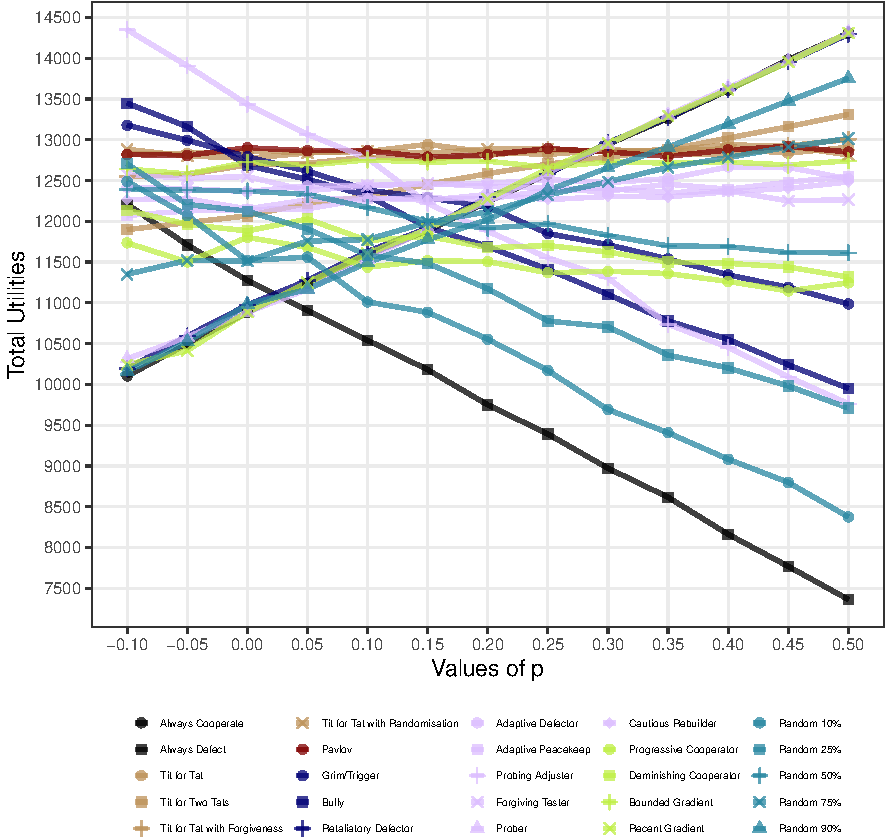
\includegraphics{Prisoners-Dilemma_files/figure-latex/unnamed-chunk-5-1} 

}

\caption{Strategies' Total Utilities for Different Strategies Accross p\label{pvalues}}\label{fig:unnamed-chunk-5}
\end{figure}

Figure \ref{pvalues} presents a graphical representation of how the
total points of different strategies change as p varies. The x-axis
represents different \emph{p} values, while the y-axis shows the total
points for each strategy. From the figure we observe that Always
Cooperate shows a steady increase in total points as \emph{p} increases,
reinforcing the observation that this strategy benefits from
environments where players value mutual cooperation. Always Defect
exhibits declining points as \emph{p} increases, suggesting that as
social preferences rise, defectors are penalized for their selfishness.
TfT maintains consistently high points across all \emph{p} values,
further proving its adaptability and effectiveness in both selfish and
cooperative environments. Strategies like Probing Adjuster and Bully,
which perform well in self-interested settings, see their points drop as
\emph{p} increases, emphasizing their reduced effectiveness in more
cooperative contexts.

\begin{table}[!h]
\centering
\caption{\label{tab:unnamed-chunk-6}Strategy Rankings Across All p-Values}
\centering
\resizebox{\ifdim\width>\linewidth\linewidth\else\width\fi}{!}{
\fontsize{8}{10}\selectfont
\begin{tabular}[t]{>{\centering\arraybackslash}p{2cm}>{\centering\arraybackslash}p{5cm}>{\centering\arraybackslash}p{3cm}}
\toprule
Ranking & Strategy & Average\\
\midrule
\textbf{1} & Tit for Tat & 12861.115\\
\textbf{2} & Pavlov & 12849.538\\
\textbf{3} & Tit for Tat with Randomisation & 12846.385\\
\textbf{4} & Tit for Tat with Forgiveness & 12797.942\\
\textbf{5} & Bounded Gradient & 12701.000\\
\textbf{6} & Tit for Two Tats & 12566.788\\
\textbf{7} & Adaptive Defector & 12487.250\\
\textbf{8} & Forgiving Tester & 12415.192\\
\textbf{9} & Adaptive Peacekeep & 12304.769\\
\textbf{10} & Cautious Rebuilder & 12303.923\\
\textbf{11} & Retaliatory Defector & 12273.365\\
\textbf{12} & Prober & 12261.308\\
\textbf{13} & Recent Gradient & 12256.058\\
\textbf{14} & Always Cooperate & 12239.635\\
\textbf{15} & Random 75\% & 12169.135\\
\textbf{16} & Grim/Trigger & 12080.481\\
\textbf{17} & Random 90\% & 12037.250\\
\textbf{18} & Random 50\% & 11997.865\\
\textbf{19} & Probing Adjuster & 11964.308\\
\textbf{20} & Deminishing Cooperator & 11717.808\\
\textbf{21} & Bully & 11674.346\\
\textbf{22} & Progressive Cooperator & 11457.731\\
\textbf{23} & Random 25\% & 11147.538\\
\textbf{24} & Random 10\% & 10431.865\\
\textbf{25} & Always Defect & 9757.308\\
\bottomrule
\end{tabular}}
\end{table}

The analysis of the tournament shows how different strategies perform in
the Prisoner's Dilemma under varying levels of social preference. The
findings yield that in selfish scenarios, probing and aggressive
strategies tend to win but as altruism increases, these strategies
struggle. TfT variant strategies have shown to be robust under varying
social preferences as can be seen in Table 4.3. Tft has the highest
average points across the differing p-values showing its robustness in
the face of differing social preferences. These findings once again
provide insight into the strength of the TfT strategy. In Prisoner's
Dilemma games where preferences may be hidden, TfT would according to
these findings perform the best.

\begin{table}[!h]
\centering
\caption{\label{tab:unnamed-chunk-7}Strategy Values Across Different p Values}
\centering
\resizebox{\ifdim\width>\linewidth\linewidth\else\width\fi}{!}{
\fontsize{5}{7}\selectfont
\begin{tabular}[t]{>{\centering\arraybackslash}p{4cm}>{\centering\arraybackslash}p{0.7cm}>{\centering\arraybackslash}p{0.7cm}>{\centering\arraybackslash}p{0.7cm}>{\centering\arraybackslash}p{0.7cm}>{\centering\arraybackslash}p{0.7cm}>{\centering\arraybackslash}p{0.7cm}>{\centering\arraybackslash}p{0.7cm}>{\centering\arraybackslash}p{0.7cm}>{\centering\arraybackslash}p{0.7cm}>{\centering\arraybackslash}p{0.7cm}>{\centering\arraybackslash}p{0.7cm}>{\centering\arraybackslash}p{0.7cm}>{\centering\arraybackslash}p{0.7cm}}
\toprule
\multicolumn{1}{c}{ } & \multicolumn{13}{c}{p Values} \\
\cmidrule(l{3pt}r{3pt}){2-14}
Strategy & -0.1 & -0.05 & 0 & 0.05 & 0.1 & 0.15 & 0.2 & 0.25 & 0.3 & 0.35 & 0.4 & 0.45 & 0.5\\
\midrule
\textbf{Always Cooperate} & 10103.5 & 10495.5 & 10881 & 11240.75 & 11585 & 11886 & 12238 & 12579.75 & 12945 & 13262.5 & 13608 & 13982.25 & 14308\\
\textbf{Always Defect} & 12209 & 11710.75 & 11276 & 10906.25 & 10540.5 & 10180.5 & 9749 & 9391.75 & 8972.5 & 8615.75 & 8162 & 7768.5 & 7362.5\\
\textbf{Tit for Tat} & 12824 & 12832 & 12863 & 12844.5 & 12856 & 12943.5 & 12845 & 12820.5 & 12875.5 & 12856.25 & 12891 & 12834.75 & 12908.5\\
\textbf{Tit for Two Tats} & 11897.5 & 11983.5 & 12067 & 12221.25 & 12304 & 12453.5 & 12584 & 12701.5 & 12786.5 & 12878.25 & 13021 & 13159.75 & 13310.5\\
\textbf{Tit for Tat with Forgiveness} & 12551 & 12573.75 & 12692 & 12711.5 & 12787.5 & 12766 & 12809 & 12878 & 12863.5 & 12874.5 & 12936 & 12926 & 13004.5\\
\midrule
\textbf{Tit for Tat with Randomisation} & 12883.5 & 12801.25 & 12772 & 12837.25 & 12864.5 & 12836.5 & 12884 & 12886.75 & 12854 & 12843.25 & 12806 & 12920.5 & 12813.5\\
\textbf{Pavlov} & 12818 & 12807.5 & 12902 & 12866.5 & 12864 & 12787.25 & 12815 & 12891.5 & 12851 & 12797.25 & 12875 & 12919.5 & 12849.5\\
\textbf{Grim/Trigger} & 13178 & 12993 & 12791 & 12613.75 & 12382 & 12289.25 & 12178 & 11850.25 & 11713.5 & 11537.75 & 11343 & 11189.75 & 10987\\
\textbf{Bully} & 13447.5 & 13160 & 12685 & 12513.75 & 12312 & 11926.25 & 11688 & 11410 & 11103 & 10778.75 & 10552 & 10240.25 & 9950\\
\textbf{Retaliatory Defector} & 10192.5 & 10593 & 10972 & 11274.25 & 11629.5 & 11915.75 & 12296 & 12581 & 12963.5 & 13270.25 & 13616 & 13955.5 & 14294.5\\
\midrule
\textbf{Adaptive Defector} & 12417.5 & 12400.25 & 12365 & 12433 & 12444.5 & 12452 & 12465 & 12511.5 & 12474.5 & 12522.75 & 12666 & 12661.75 & 12520.5\\
\textbf{Adaptive Peacekeep} & 12071.5 & 12127 & 12145 & 12154.5 & 12277 & 12286.75 & 12271 & 12382 & 12370 & 12455.5 & 12393 & 12479.75 & 12549\\
\textbf{Probing Adjuster} & 14349.5 & 13907 & 13434 & 13067 & 12773.5 & 12220.5 & 11878 & 11552.25 & 11306 & 10737.25 & 10455 & 10093.5 & 9762.5\\
\textbf{Forgiving Tester} & 12574 & 12528 & 12549 & 12374.5 & 12437 & 12464.5 & 12427 & 12404 & 12399.5 & 12352.25 & 12372 & 12251.25 & 12264.5\\
\textbf{Prober} & 10313.5 & 10580 & 10884 & 11166.5 & 11537.5 & 11910.75 & 12248 & 12593.75 & 12948 & 13302.5 & 13637 & 13962 & 14313.5\\
\midrule
\textbf{Cautious Rebuilder} & 12268.5 & 12276.25 & 12152 & 12263.5 & 12287 & 12258.25 & 12329 & 12265.5 & 12303.5 & 12299 & 12363 & 12403 & 12482.5\\
\textbf{Progressive Cooperator} & 11735.5 & 11501.25 & 11803 & 11680.25 & 11437.5 & 11518.25 & 11505 & 11369 & 11387.5 & 11359.5 & 11262 & 11146.25 & 11245.5\\
\textbf{Deminishing Cooperator} & 12135 & 11963.25 & 11882 & 12028 & 11763.5 & 11817 & 11676 & 11703 & 11622.5 & 11501.75 & 11485 & 11439 & 11315.5\\
\textbf{Bounded Gradient} & 12641.5 & 12580.75 & 12724 & 12688.75 & 12752.5 & 12726.5 & 12737 & 12661.25 & 12728.5 & 12713.75 & 12727 & 12690 & 12741.5\\
\textbf{Recent Gradient} & 10240 & 10414.25 & 10887 & 11246.25 & 11602.5 & 11904 & 12272 & 12642.75 & 12951 & 13291.25 & 13613 & 13953.75 & 14311\\
\midrule
\textbf{Random 10\%} & 12488 & 12072.5 & 11518 & 11561 & 11011 & 10884.75 & 10554 & 10170.75 & 9691.5 & 9407 & 9083 & 8798.25 & 8374.5\\
\textbf{Random 25\%} & 12705.5 & 12206.75 & 12123 & 11906 & 11585 & 11484 & 11173 & 10777.75 & 10706 & 10359.75 & 10201 & 9980.25 & 9710\\
\textbf{Random 50\%} & 12391.5 & 12384.25 & 12371 & 12330.25 & 12168 & 12000 & 11914 & 11968.5 & 11827.5 & 11699.25 & 11690 & 11614.5 & 11613.5\\
\textbf{Random 75\%} & 11350 & 11521 & 11512 & 11756.75 & 11776 & 11989.25 & 12117 & 12323 & 12484 & 12661.25 & 12782 & 12911 & 13015.5\\
\textbf{Random 90\%} & 10159.5 & 10523.5 & 10980 & 11167.75 & 11493 & 11775.25 & 12019 & 12379.75 & 12656.5 & 12909.5 & 13192 & 13475 & 13753.5\\
\bottomrule
\end{tabular}}
\end{table}

\section{Conclusion}\label{conclusion}

The tournament results reveal that strategic success in the Prisoner's
Dilemma is highly dependent on the composition of competing strategies
and the level of social preferences. Probing Adjuster outperformed other
strategies in the standard setting, but TfT and its variants
demonstrated remarkable robustness across different social preference
levels. As altruism increases, cooperative strategies gain prominence,
while aggressive strategies struggle. The findings highlight the
continued relevance of TfT, particularly in contexts where social
preferences or hidden intentions influence decision-making, offering
valuable insights into strategic adaptability in competitive
environments.

\newpage

\section*{References}\label{references}
\addcontentsline{toc}{section}{References}

\phantomsection\label{refs}
\begin{CSLReferences}{1}{1}
\bibitem[\citeproctext]{ref-axelrod1980effective}
Axelrod, R. 1980. Effective choice in the prisoner's dilemma. \emph{The
Journal of Conflict Resolution}. 24(1):3--25. {[}Online{]}, Available:
\url{http://www.jstor.org/stable/173932}.

\bibitem[\citeproctext]{ref-dalbo2019strategy}
Bó, P.D. \& Fréchette, G.R. 2019.
\href{https://doi.org/10.1257/aer.20181480}{Strategy choice in the
infinitely repeated prisoner's dilemma}. \emph{American Economic
Review}. 109(11):3929--3952.

\bibitem[\citeproctext]{ref-breitmoser2015cooperation}
Breitmoser, Y. 2015.
\href{https://doi.org/10.1257/aer.20130675}{Cooperation, but no
reciprocity: Individual strategies in the repeated prisoner's dilemma}.
\emph{American Economic Review}. 105(9):2882--2910.

\bibitem[\citeproctext]{ref-charness2002understanding}
Charness, G. \& Rabin, M. 2002. Understanding social preferences with
simple tests. \emph{The quarterly journal of economics}.
117(3):817--869.

\bibitem[\citeproctext]{ref-embrey2017cooperation}
Embrey, M., Fréchette, G.R. \& Yuksel, S. 2018.
\href{https://doi.org/10.1093/qje/qjx033}{Cooperation in the finitely
repeated prisoner's dilemma}. \emph{The Quarterly Journal of Economics}.
133(2):509--551.

\bibitem[\citeproctext]{ref-farrell1988evolutionary}
Farrell, J. \& Ware, R. 1989. Evolutionary stability in the repeated
prisoner's dilemma. \emph{Journal of Economic Theory}. 47(1):1--12.

\bibitem[\citeproctext]{ref-garcia2018no}
García, J. \& Veelen, M. van. 2018.
\href{https://doi.org/10.3389/frobt.2018.00102}{No strategy can win in
the repeated prisoner's dilemma: Linking game theory and computer
simulations}. \emph{Frontiers in Robotics and AI}. 5:102.

\bibitem[\citeproctext]{ref-gaudesi2016exploiting}
Gaudesi, M., Piccolo, E., Squillero, G. \& Tonda, A. 2016. Exploiting
evolutionary modeling to prevail in iterated prisoner's dilemma
tournaments. \emph{IEEE Transactions on Computational Intelligence and
AI in Games}. 8(3):235--247.

\bibitem[\citeproctext]{ref-kreps1982rational}
Kreps, D.M., Milgrom, P., Roberts, J. \& Wilson, R. 1982. Rational
cooperation in the finitely repeated prisoners' dilemma. \emph{Journal
of Economic Theory}. 27(2):245--252.

\bibitem[\citeproctext]{ref-lange2007teaching}
Lange, C. \& Baylor, A.L. 2007.
\href{https://doi.org/10.3200/JECE.38.4.407-418}{Teaching the repeated
prisoner's dilemma with a computerized tournament}. \emph{The Journal of
Economic Education}. 38(4):407--418.

\bibitem[\citeproctext]{ref-romero2018constructing}
Romero, J. \& Rosokha, Y. 2018.
\href{https://doi.org/10.1016/j.euroecorev.2018.02.008}{Constructing
strategies in the indefinitely repeated prisoner's dilemma game}.
\emph{European Economic Review}. 104:185--219.

\end{CSLReferences}

\bibliography{Tex/ref}





\end{document}
